\documentclass{article}
\usepackage[T1]{fontenc}
\usepackage{lmodern}
\usepackage{amsmath,amssymb}
\usepackage{tikz}
\usepackage[margin=1in]{geometry}

% --- importer markers (no-ops for LaTeX; used by your importer) ---
\newenvironment{asset}[1]{}{}   % wraps a shared figure/table; #1 = asset key
\newcommand{\uses}[1]{}         % mark items that consume that asset

\begin{document}

%========= Shared assets (parsed by importer) ===================================

% Strep/Healthy 2x2 table used by S1–S4
\begin{asset}{strep-2x2}
\begin{center}
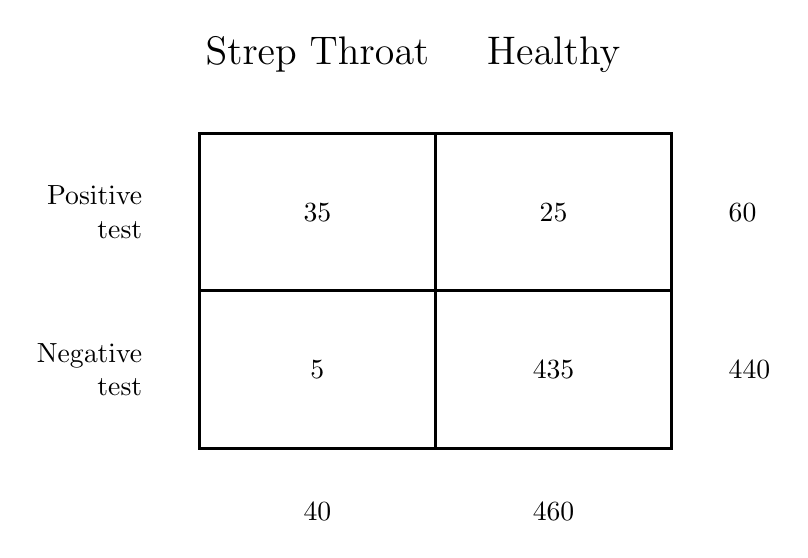
\begin{tikzpicture}[x=1cm,y=1cm]
  % Column titles
  \node[font=\Large] at (1.5,5.0) {Strep Throat};
  \node[font=\Large] at (4.5,5.0) {Healthy};

  % Outer 2x2 box and dividers
  \draw[line width=1pt] (0,0) rectangle (6,4);
  \draw[line width=1pt] (3,0) -- (3,4);
  \draw[line width=1pt] (0,2) -- (6,2);

  % Cell counts
  \node at (1.5,3) {35};
  \node at (4.5,3) {25};
  \node at (1.5,1) {5};
  \node at (4.5,1) {435};

  % Row labels (left of box)
  \node[anchor=east,align=right] at (-0.6,3) {Positive\\test};
  \node[anchor=east,align=right] at (-0.6,1) {Negative\\test};

  % Row totals (to the right of box)
  \node[anchor=west] at (6.6,3) {60};
  \node[anchor=west] at (6.6,1) {440};

  % Column totals (below box)
  \node at (1.5,-0.8) {40};
  \node at (4.5,-0.8) {460};
\end{tikzpicture}
\end{center}
\end{asset}

\bigskip
%===============================================================================

% (Example) Mosaic plot as a separate asset (attach via \uses{mosaic-tattoos-college} in the relevant item)
A random sample of adults aged 25 and up were surveyed as to whether or not
they had tattoos and whether or not they had ever taken a college course.
The mosaic plot below displays the data.

\begin{asset}{mosaic-tattoos-college}
\begin{center}
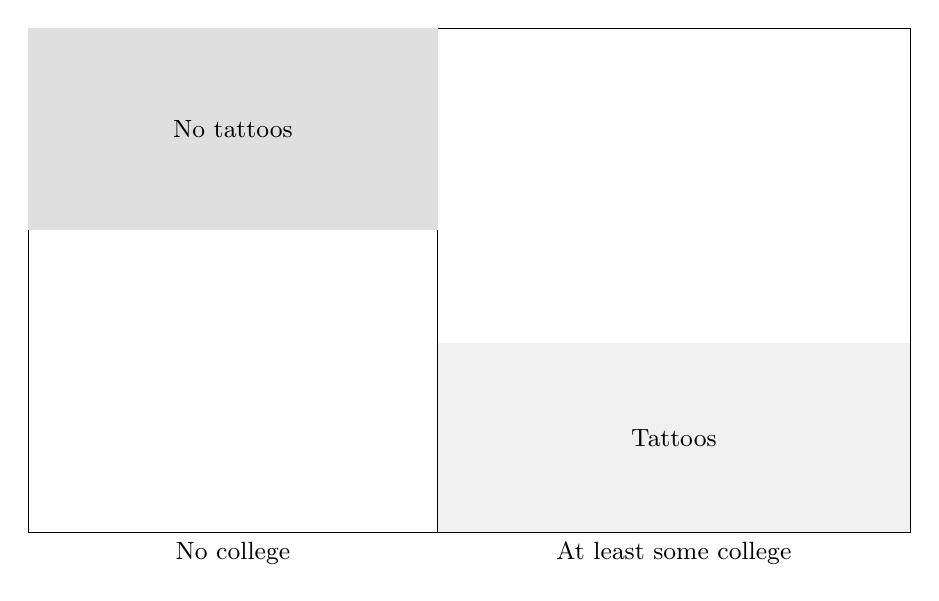
\begin{tikzpicture}[x=0.08cm,y=0.08cm,baseline]
  \draw (0,0) rectangle (140,80);
  \draw (65,0) -- (65,80);
  \draw (0,48) -- (65,48);     % left column horizontal split
  \draw (65,30) -- (140,30);   % right column horizontal split

  \fill[gray!25] (0,48) rectangle (65,80);    % No tattoos (left–top)
  \fill[gray!12] (65,0) rectangle (140,30);   % Tattoos (right–bottom)

  \node at (32.5,64) {\small No tattoos};
  \node at (102.5,15) {\small Tattoos};

  \node[below] at (32.5,0) {\small No college};
  \node[below] at (102.5,0) {\small At least some college};
\end{tikzpicture}
\end{center}
\end{asset}

Which is greater, the probability that someone in this sample has taken a college
course \emph{given} that they have a tattoo, or the probability that someone has
a tattoo \emph{given} that they have taken a college course?

%===============================================================================

\begin{enumerate}[label=\textbf{S\arabic*.}]

% --- S1 ------------------------------------------------------------------------
\item \uses{strep-2x2} \textbf{Predictive value.} What is the probability that a person has strep
throat \emph{and} tests positive? \answer{B}

\textit{Use the same table above.}

\begin{enumerate}
  \item $\dfrac{35}{500}$
  \item $\dfrac{35}{60}$
  \item $\dfrac{35}{40}$
  \item $\dfrac{35}{35+25+5}$
  \item $\dfrac{35+25+5}{500}$
\end{enumerate}

% --- S2 ------------------------------------------------------------------------
\item \uses{strep-2x2} \textbf{False-positive rate.} What is the probability of testing positive
\emph{given} that the person does \emph{not} have strep throat? \answer{A}

\textit{Use the same table above.}

\begin{enumerate}
  \item $\dfrac{25}{460}$
  \item $\dfrac{25}{60}$
  \item $\dfrac{35}{40}$
  \item $\dfrac{25}{500}$
  \item $\dfrac{35+25+5}{500}$
\end{enumerate}

% --- S3 ------------------------------------------------------------------------
\item \uses{strep-2x2} \textbf{Sensitivity.} What is the probability of testing positive
\emph{given} that the person \emph{has} strep throat? \answer{D}

\textit{Use the same table above.}

\begin{enumerate}
  \item $\dfrac{35+25+5}{500}$
  \item $\dfrac{35}{35+25+5}$
  \item $\dfrac{35}{500}$
  \item $\dfrac{35}{60}$
  \item $\dfrac{35}{40}$
\end{enumerate}

% --- S4 ------------------------------------------------------------------------
\item \uses{strep-2x2} \textbf{Specificity.} What is the probability of testing negative
\emph{given} that the person does \emph{not} have strep throat? \answer{E}

\textit{Use the same table above.}

\begin{enumerate}
  \item $\dfrac{5}{40}$
  \item $\dfrac{35}{60}$
  \item $\dfrac{35+5+435}{500}$
  \item $\dfrac{435}{500}$
  \item $\dfrac{435}{460}$
\end{enumerate}

% --- 5 (no shared asset) -------------------------------------------------------
\item In a 1974 ``Dear Abby'' letter, a woman lamented that she had just given
birth to her eighth child and all were girls. Her doctor had assured her that
the chance of the eighth child being a girl was less than $1$ in $100$.
What is the real probability that the eighth child would be a girl?
\begin{enumerate}
  \item $0.0039$
  \item $0.5$
  \item $(0.5)^{7}$
  \item $(0.5)^{8}$
  \item $\dfrac{(0.5)^{7}+(0.5)^{8}}{2}$
\end{enumerate}

% 6 --------------------------------------------------------------------------
\item Hospital A has about 20 births per day, and Hospital B has about 40 births
per day. About 50\% of all babies are boys, but the percentage who are boys
varies at each hospital from day to day. Over the course of a year, which
hospital will have more days on which 60\% or more of the births are boys?
\begin{enumerate}
  \item Hospital A
  \item Hospital B
  \item The difference will be negligible.
  \item By the law of small numbers, this cannot be predicted.
  \item By the law of large numbers, this cannot be predicted.
\end{enumerate}

% 7 --------------------------------------------------------------------------
\item The probability that a college's mathematics department will fill an opening
with a female professor is $0.55$, while the probability that the physics
department will fill an opening with a female professor is $0.3$.
Assuming independence, what is the probability that \emph{exactly one}
of these two departments will fill their position with a female professor?
\begin{enumerate}
  \item $(0.55)(0.3)$
  \item $0.55+0.3-(0.55)(0.3)$
  \item $0.55-(0.55)(0.3)$
  \item $(0.55)(0.70)+(0.30)(0.45)$
  \item $(0.55)(0.70)+(0.30)(0.45)-(0.55)(0.30)$
\end{enumerate}

% 8 --------------------------------------------------------------------------
\item Suppose that 2\% of a clinic's patients are known to have cancer.
A blood test is positive in 98\% of patients with cancer but is also positive
in 3\% of patients who do not have cancer.
If a randomly chosen patient tests positive, what is the probability
that the person actually has cancer?
\begin{enumerate}
  \item $0.02$
  \item $0.02+0.03$
  \item $(0.02)(0.98)$
  \item $(0.02)(0.98)+(0.98)(0.03)$
  \item $\displaystyle
          \frac{0.02\cdot0.98}{\,0.02\cdot0.98+0.98\cdot0.03\,}$
\end{enumerate}

% 9 --------------------------------------------------------------------------
\item A teacher has 90 students. Of those, 21 have at least two analog clocks
in their homes, and 62 have at least three television sets in their homes.
There are 15 students who do not have at least two analog clocks and do not have
at least three television sets. Let $C$ be the event “at least two analog clocks”
and $T$ the event “at least three television sets”.
Are $C$ and $T$ mutually exclusive events?
\begin{enumerate}
  \item No, because $P(C\cap T)=\dfrac{8}{90}$.
  \item No, because $P(C\cap T)=\dfrac{75}{90}$.
  \item No, because $P(C\cap T)=\dfrac{83}{90}$.
  \item Yes, because $P(C\cap T)=\dfrac{8}{90}$.
  \item Yes, because $P(C\cap T)=\dfrac{83}{90}$.
\end{enumerate}

% 10 -------------------------------------------------------------------------
\item A random sample of adults aged 25 and up were surveyed as to whether or not
they had tattoos and whether or not they had ever taken a college course.
The mosaic plot below displays the data.

\begin{center}
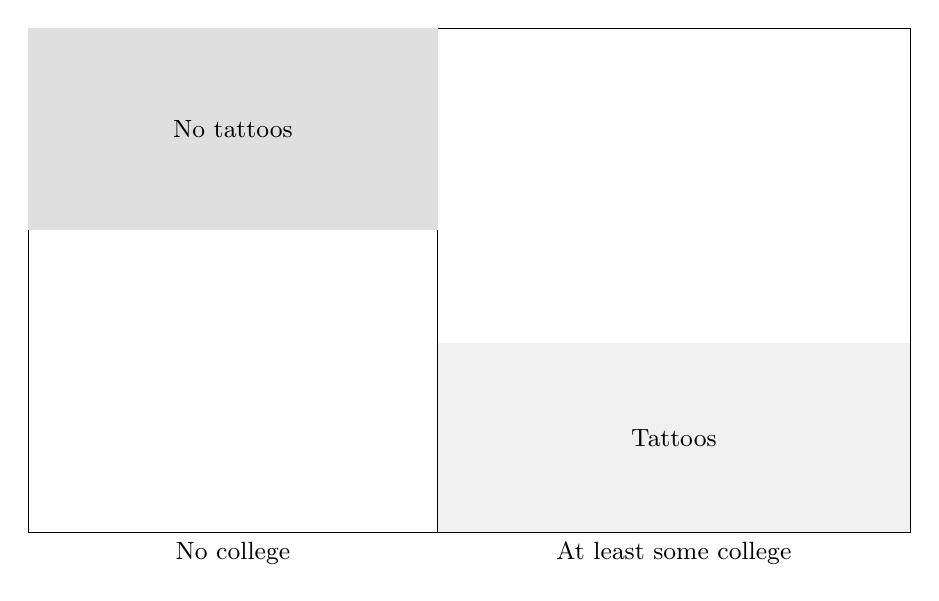
\begin{tikzpicture}[x=0.08cm,y=0.08cm,baseline]
  % total frame (width 140, height 80 for easy ratios)
  \draw (0,0) rectangle (140,80);
  % column split (adjust 65/75 if you want different column totals)
  \draw (65,0) -- (65,80);
  % row splits within each column (adjust 48 and 30 to change row proportions)
  \draw (0,48) -- (65,48);     % left column horizontal split
  \draw (65,30) -- (140,30);   % right column horizontal split

  % subtle shading to differentiate blocks (tune to taste)
  \fill[gray!25] (0,48) rectangle (65,80);    % No tattoos (left–top)
  \fill[gray!12] (65,0) rectangle (140,30);   % Tattoos (right–bottom)

  % labels inside/under
  \node at (32.5,64) {\small No tattoos};
  \node at (102.5,15) {\small Tattoos};

  \node[below] at (32.5,0) {\small No college};
  \node[below] at (102.5,0) {\small At least some college};
\end{tikzpicture}
\end{center}

Which is greater, the probability that someone in this sample has taken a college
course \emph{given} that they have a tattoo, or the probability that someone has
a tattoo \emph{given} that they have taken a college course?
\begin{enumerate}
  \item The probability of college $\mid$ tattoo is greater.
  \item The probability of tattoo $\mid$ college is greater.
  \item The two probabilities are equal.
  \item This cannot be answered without knowing $P(\text{college and tattoo})$.
  \item This cannot be answered without knowing
        (1) $P(\text{college})$, (2) $P(\text{tattoo})$, and
        (3) $P(\text{college and tattoo})$.
\end{enumerate}

% 11 -------------------------------------------------------------------------
\item For which of the following probability assignments are events $E$ and $F$
independent? (Each row lists $P(E\cap F^{c})$, $P(E\cap F)$, $P(E^{c}\cap F)$;
the remaining cell is $P(E^{c}\cap F^{c})=1$ minus the sum of those three.)
\begin{enumerate}
  \item $0.2,\;0.2,\;0.2$
  \item $0.3,\;0.0,\;0.3$
  \item $0.3,\;0.2,\;0.1$
  \item $0.4,\;0.1,\;0.1$
  \item $0.2,\;0.4,\;0.2$
\end{enumerate}

% 12 -------------------------------------------------------------------------
\item What is the proper order of size for the probabilities of the following three events?
\begin{itemize}
  \item[I.] A randomly selected high school senior eats breakfast.
  \item[II.] A randomly selected \emph{teenager} is a high school senior who eats breakfast.
  \item[III.] A randomly selected teenager who eats breakfast is a high school senior.
\end{itemize}
Which order best compares these probabilities?
\begin{enumerate}
  \item $P(\text{I})<P(\text{II})<P(\text{III})$
  \item $P(\text{I})>P(\text{II})>P(\text{III})$
  \item $P(\text{I})<P(\text{III})<P(\text{II})$
  \item $P(\text{I})>P(\text{III})>P(\text{II})$
  \item $P(\text{II})<P(\text{I})<P(\text{III})$
\end{enumerate}

\item An insurance company charges \$800 annually for car insurance. The policy specifies that the company will pay \$1,000 for a minor accident and \$5,000 for a major accident. If the probability of a motorist having a minor accident during the year is $0.2$ and of having a major accident is $0.05$, how much can the insurance company expect to make on a policy? \answer{D}
\begin{enumerate}
  \item \$200
  \item \$250
  \item \$300
  \item \$350
  \item \$450
\end{enumerate}

\item Suppose you are one of $7.5$ million people who send in their name for a drawing with $1$ top prize of \$1,000,000, five second-place prizes of \$10,000, and $20$ third-place prizes of \$100. Is it worth the \$0.66 postage it costs you to send in your name? \answer{B}
\begin{enumerate}
  \item Yes, because $\dfrac{1,000,000}{0.66} = 1,515,152$, which is less than $7,500,000$.
  \item No, because your expected winnings are only $0.14$.
  \item Yes, because $\dfrac{7,500,000}{1+5+20} = 288,642$.
  \item No, because $1,052,000 < 7,500,000$.
  \item Yes, because $\dfrac{1,052,000}{26} = 40,462$.
\end{enumerate}

\item The random variable $X$ has mean $15$ and standard deviation $4$. The random variable $Y$ is defined by $Y=3+2X$. What are the mean and standard deviation of $Y$? \answer{D}
\begin{enumerate}
  \item The mean is $30$, and the standard deviation is $8$.
  \item The mean is $30$, and the standard deviation is $11$.
  \item The mean is $33$, and the standard deviation is $4$.
  \item The mean is $33$, and the standard deviation is $8$.
  \item The mean is $33$, and the standard deviation is $11$.
\end{enumerate}

\item Each hospital Internet security breach results in the theft of an average of $361$ patient records with a standard deviation of $74$ records. If there are $45$ independent breaches during a one-year period, what is the expected value and standard deviation for the \emph{total} number of patient records stolen? \answer{C}
\begin{enumerate}
  \item $E(\text{thefts})=\sqrt{45}\times361$ $SD(\text{thefts})=\sqrt{45}\times74$
  \item $E(\text{thefts})=\sqrt{45}\times361$ $SD(\text{thefts})=45\times74$
  \item $E(\text{thefts})=45\times361$ $SD(\text{thefts})=\sqrt{45}\times74$
  \item $E(\text{thefts})=45\times361$ $SD(\text{thefts})=45\times74$
  \item $E(\text{thefts})=45\times361$ $SD(\text{thefts})=45\times74^{2}$
\end{enumerate}

\item The auditor working for a veterinary clinic calculates that the mean annual cost of medical care for dogs is \$98 with a standard deviation of \$25 and that the mean annual cost of medical care for a dog–cat household (one dog and one cat) is \$212 with a standard deviation of \$39. Assuming expenses for dogs and cats are independent for such households, what are the mean annual cost of medical care for \emph{cats} and its standard deviation? \answer{C}
\begin{enumerate}
  \item $E(\text{Cats})=\$114$ $SD(\text{Cats})=\$14$
  \item $E(\text{Cats})=\$114$ $SD(\text{Cats})=\$46$
  \item $E(\text{Cats})=\$114$ $SD(\text{Cats})=\$30$
  \item $E(\text{Cats})=\$155$ $SD(\text{Cats})=\$32$
  \item $E(\text{Cats})=\$188$ $SD(\text{Cats})=\$30$
\end{enumerate}

\item Boxes of $50$ donut holes weigh an average of $16.0$ ounces with a standard deviation of $0.245$ ounces. The empty boxes alone weigh an average of $1.0$ ounce with a standard deviation of $0.2$ ounces. What are the mean and standard deviation of the \emph{total donut-hole weight per box}? (Assume independence of box and contents.) \answer{D}
\begin{enumerate}
  \item $E(\text{Donut hole})=0.3\ \text{oz}$ $SD(\text{Donut hole})=0.0063\ \text{oz}$
  \item $E(\text{Donut hole})=0.3\ \text{oz}$ $SD(\text{Donut hole})=0.02\ \text{oz}$
  \item $E(\text{Donut hole})=0.3\ \text{oz}$ $SD(\text{Donut hole})=0.142\ \text{oz}$
  \item $E(\text{Donut hole})=15\ \text{oz}$ $SD(\text{Donut hole})=0.142\ \text{oz}$
  \item $E(\text{Donut hole})=15\ \text{oz}$ $SD(\text{Donut hole})=0.445\ \text{oz}$
\end{enumerate}

% --- New Set -------------------------------------------------------------

\item An inspection procedure at a manufacturing plant involves picking three items at random and then accepting the whole lot if at least two of the three items are in perfect condition. If in reality $90\%$ of the whole lot are perfect, what is the probability that the lot will be accepted? \answer{E}

\begin{enumerate}
  \item $3(0.1)^2(0.9)$
  \item $3(0.9)^2(0.1)$
  \item $(0.1)^3 + (0.1)^2(0.9)$
  \item $(0.1)^3 + 3(0.1)^2(0.9)$
  \item $(0.9)^3 + 3(0.9)^2(0.1)$
\end{enumerate}

\item Suppose we have a random variable $X$ where, for the values $k=0,\dots,10$, the associated probabilities are $\binom{10}{k}(0.37)^k(0.63)^{10-k}$. What is the mean of $X$? \answer{C}

\begin{enumerate}
  \item $0.37$
  \item $0.63$
  \item $3.7$
  \item $6.3$
  \item None of the above
\end{enumerate}

\item One in six adults in the workplace has experienced cyberbullying. In a random sample of five adults in the workplace, what is the distribution for the number who have experienced cyberbullying? \answer{B}

\begin{enumerate}
  \item Binomial with $n=6$ and $p=\tfrac{1}{6}$
  \item Binomial with $n=5$ and $p=\tfrac{1}{6}$
  \item Binomial with $n=5$ and $p=\tfrac{1}{5}$
  \item Geometric with $p=\tfrac{1}{6}$
  \item Geometric with $p=\tfrac{1}{5}$
\end{enumerate}

% Q4–Q5 shared context
\item It is estimated that two out of five high school students would fall victim to a phishing email (an online scam asking for sensitive information) if it appears to originate from their high school main office.

In a random sample of five high school students, what is the probability that exactly two fall victim to a phishing email that appears to originate from their high school main office? \answer{C}

\begin{enumerate}
  \item $0.4$
  \item $1.0$
  \item $\binom{5}{2}(0.4)^2(0.6)^3$
  \item $\binom{5}{2}(0.4)^3(0.6)^2$
  \item $(0.4)^2(0.6)^3$
\end{enumerate}

\item What is the probability that the first student to fall victim will be the third student who is sent a phishing email that appears to originate from their high school main office? \answer{D}

\begin{enumerate}
  \item $(0.4)^3$
  \item $(0.6)^3$
  \item $(0.6)(0.4)^2$
  \item $(0.6)^2(0.4)$
  \item $10(0.6)^2(0.4)$
\end{enumerate}

\item Suppose that one out of 20 apples from a particular orchard is wormy. What are the mean and standard deviation for the number of apples to be sampled from this orchard before finding a wormy apple? (Let the count start at $1$ for the first apple picked.) \answer{D}

\begin{enumerate}
  \item Mean $=5$, standard deviation $=1$
  \item Mean $=5$, standard deviation $=1-0.05$
  \item Mean $=10$, standard deviation $=\sqrt{\dfrac{(0.05)^2}{1-0.05}}$
  \item Mean $=20$, standard deviation $=\sqrt{380}$
  \item Mean $=20$, standard deviation $=\sqrt{\dfrac{1-0.95}{(0.95)^2}}$
\end{enumerate}

\item A fair coin is flipped 5 times. Consider the following 3 outcomes where H refers to a toss resulting in “heads” and T refers to a toss resulting in “tails”:

\begin{itemize}
  \item[I.] The result in order is HHTTT.
  \item[II.] The result in order is HTTHH.
  \item[III.] The result includes 3 Hs and 2 Ts.
\end{itemize}

What is a comparison of the three probabilities? \answer{D}

\begin{enumerate}
  \item $P(\mathrm{I}) < P(\mathrm{II}) < P(\mathrm{III})$
  \item $P(\mathrm{II}) < P(\mathrm{I}) < P(\mathrm{III})$
  \item $P(\mathrm{III}) < P(\mathrm{I}) < P(\mathrm{II})$
  \item $P(\mathrm{I}) = P(\mathrm{II}) < P(\mathrm{III})$
  \item $P(\mathrm{III}) < P(\mathrm{I}) = P(\mathrm{II})$
\end{enumerate}

\item A statistician working for an online dating service determines that the binomial random variable $D$, representing the number of people in a sample who are happy with the service, has a mean of $5$ with a standard deviation of $2$. What is the probability that someone is happy with the service? \answer{B}

\begin{enumerate}
  \item $0.1$
  \item $0.2$
  \item $0.4$
  \item $0.6$
  \item $0.8$
\end{enumerate}

% Histogram asset for Q9
\begin{asset}{binom-07-n10-hists}
\begin{center}
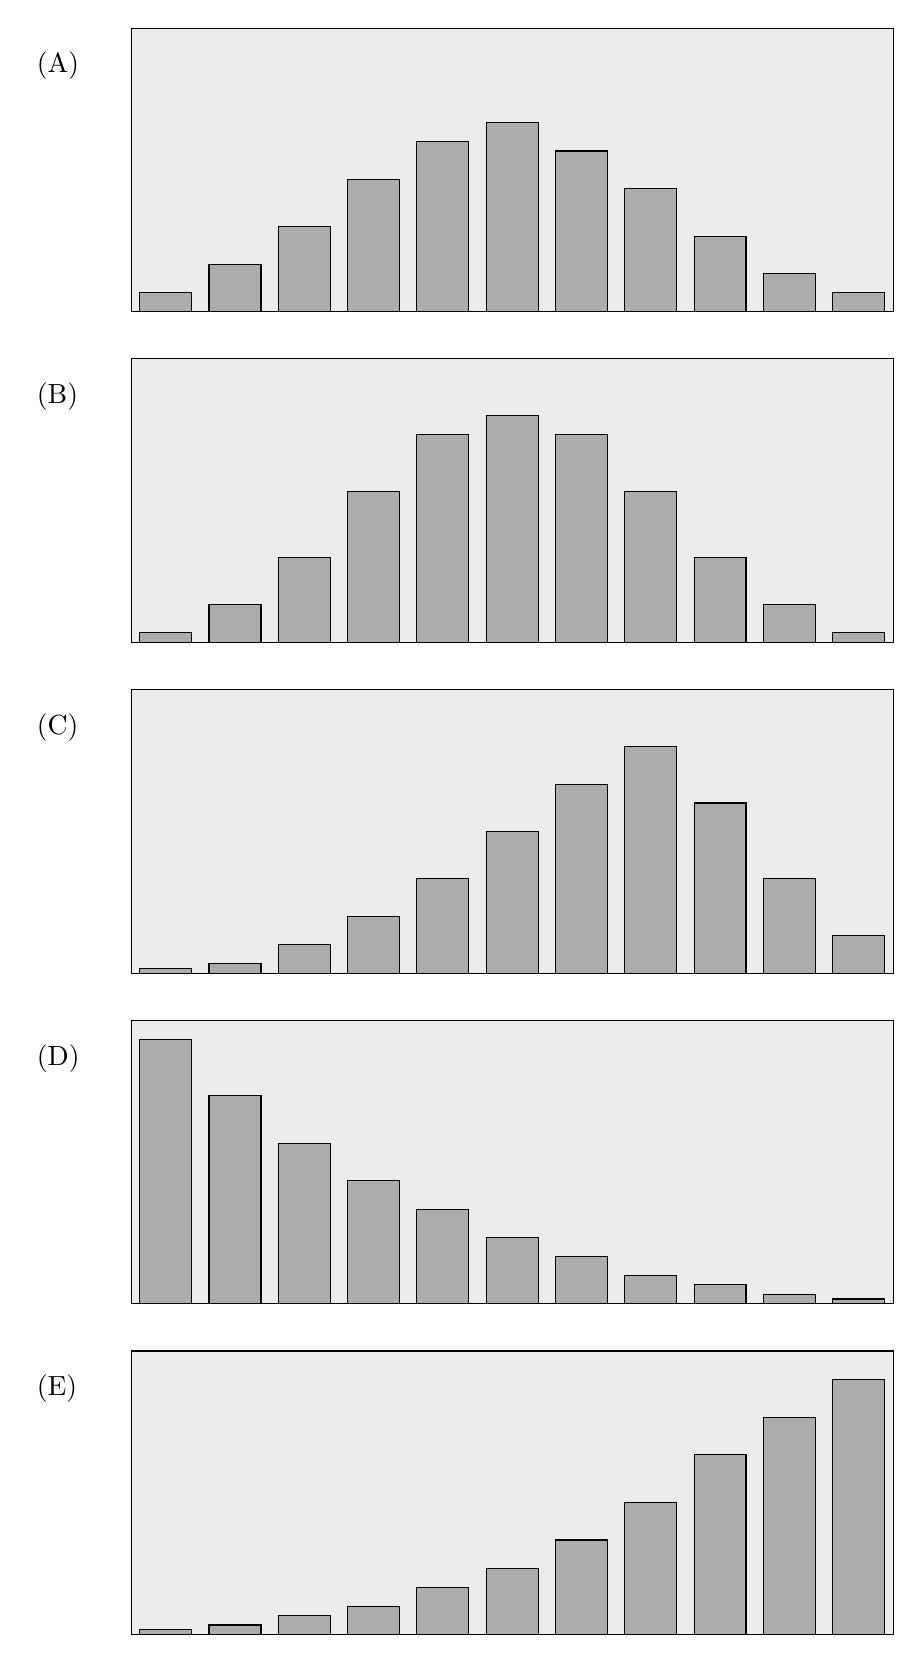
\begin{tikzpicture}[x=0.22cm,y=0.12cm]
  \def\panel#1#2#3{
    \begin{scope}[shift={(#1,#2)}]
      \draw[fill=gray!15,draw=none] (0,0) rectangle (44,30);
      \draw (0,0) rectangle (44,30);
      \node[anchor=west] at (-6,26) {#3};
    \end{scope}
  }
  % A (roughly centered near 5, moderate spread)
  \panel{0}{90}{(A)}
  \foreach \k/\h in {0/2,1/5,2/9,3/14,4/18,5/20,6/17,7/13,8/8,9/4,10/2} {
    \draw[fill=gray!65] (0.5+4*\k,90) rectangle (0.5+4*\k+3,90+\h);
  }
  % B (symmetric around 5, taller)
  \panel{0}{55}{(B)}
  \foreach \k/\h in {0/1,1/4,2/9,3/16,4/22,5/24,6/22,7/16,8/9,9/4,10/1} {
    \draw[fill=gray!65] (0.5+4*\k,55) rectangle (0.5+4*\k+3,55+\h);
  }
  % C (center near 7: correct for p=0.7)
  \panel{0}{20}{(C)}
  \foreach \k/\h in {0/0.5,1/1,2/3,3/6,4/10,5/15,6/20,7/24,8/18,9/10,10/4} {
    \draw[fill=gray!65] (0.5+4*\k,20) rectangle (0.5+4*\k+3,20+\h);
  }
  % D (monotonically decreasing)
  \panel{0}{-15}{(D)}
  \foreach \k/\h in {0/28,1/22,2/17,3/13,4/10,5/7,6/5,7/3,8/2,9/1,10/0.5} {
    \draw[fill=gray!65] (0.5+4*\k,-15) rectangle (0.5+4*\k+3,-15+\h);
  }
  % E (monotonically increasing)
  \panel{0}{-50}{(E)}
  \foreach \k/\h in {0/0.5,1/1,2/2,3/3,4/5,5/7,6/10,7/14,8/19,9/23,10/27} {
    \draw[fill=gray!65] (0.5+4*\k,-50) rectangle (0.5+4*\k+3,-50+\h);
  }
\end{tikzpicture}
\end{center}
\end{asset}

\item \uses{binom-07-n10-hists}
A college lecture class has 500 students, of which 350 are female. Let the random variable $F$ represent the number of females in a random sample of 10 students from the class. Distribution $F$ is binomial with $n=10$ and $p=0.7$. A simulation of $F$ is performed by randomly picking 10 students from this class a large number of times. Which of the following histograms best represents this simulation? \answer{C}

\begin{enumerate}
  \item (A)
  \item (B)
  \item (C)
  \item (D)
  \item (E)
\end{enumerate}

\item If it was possible, would you want to live forever? When asked, $34\%$ of people answer yes. Let the random variable $L$ represent the number of people who would answer yes in a random sample of 50 people. Random variable $L$ follows a binomial distribution with a mean of $17$ and a standard deviation of $3.35$. Which of the following is the best interpretation of the mean? \answer{D}

\begin{enumerate}
  \item Every random sample of 50 people will have $34\%$ answering yes.
  \item Every random sample of 50 people will have $34\%$ answering no.
  \item On average, 17 people will have to be surveyed before finding one who answers yes.
  \item In repeated random sampling of 50 people, the average number of people answering yes is $17$.
  \item In repeated random sampling of 50 people, the average number of people answering yes will vary from $17$ by an average of $3.35$.
\end{enumerate}

\item Seventy percent of American households own an outdoor grill. Let the random variable $G$ represent the number of randomly selected households surveyed to find one with an outdoor grill. Which of the following is the best interpretation of the mean of $G$? \answer{C}

\begin{enumerate}
  \item A value randomly selected from the distribution of $G$ is expected to be $1.43$.
  \item In repeated sampling from the distribution of $G$, the average of the values will approach $0.7$.
  \item In repeated sampling from the distribution of $G$, the average of the values will approach $1.43$.
  \item The probability is $0.7$ that a value randomly selected from the distribution of $G$ will be close to $1.43$.
  \item For a sample of values randomly selected from the distribution of $G$, the average of the sample will vary from $1.43$ by an average of $0.782$.
\end{enumerate}



\end{enumerate}

\end{document}








    









